\documentclass{article}

% if you need to pass options to natbib, use, e.g.:
%     \PassOptionsToPackage{numbers, compress}{natbib}
% before loading neurips_2020

% ready for submission
% \usepackage{neurips_2020}

% to compile a preprint version, e.g., for submission to arXiv, add add the
% [preprint] option:
    \usepackage[final, nonatbib, preprint]{neurips_2021}

% to compile a camera-ready version, add the [final] option, e.g.:
%     \usepackage[final]{neurips_2020}

% to avoid loading the natbib package, add option nonatbib:
 %    \usepackage[nonatbib]{neurips_2020}

\usepackage[utf8]{inputenc} % allow utf-8 input
\usepackage[T1]{fontenc}    % use 8-bit T1 fonts
\usepackage{hyperref}       % hyperlinks
\usepackage{url}            % simple URL typesetting
\usepackage{booktabs}       % professional-quality tables
\usepackage{amsfonts}       % blackboard math symbols
\usepackage{nicefrac}       % compact symbols for 1/2, etc.
\usepackage{microtype}      % microtypography
\usepackage{graphicx,wrapfig,lipsum}
\usepackage{floatrow}
\usepackage{subfig}
\usepackage{amsmath}
\usepackage{wrapfig}
\usepackage{siunitx}

\usepackage[ 
	backend=bibtex8,     
    style=authoryear,	
    maxcitenames=2,      
    maxbibnames=25,  
    dashed = false,		
    hyperref=true,       
    bibencoding=inputenc,   
    useeditor=false,  
    uniquename=init,  
    doi=true,
    url=false,
    isbn = false,
    giveninits = true,
    natbib=true
]{biblatex}
	
\addbibresource{literature.bib}

\title{Medical Drug Review Analysis}

% The \author macro works with any number of authors. There are two commands
% used to separate the names and addresses of multiple authors: \And and \AND.
%
% Using \And between authors leaves it to LaTeX to determine where to break the
% lines. Using \AND forces a line break at that point. So, if LaTeX puts 3 of 4
% authors names on the first line, and the last on the second line, try using
% \AND instead of \And before the third author name.

\author{%
  Simon Reif\\
  Matrikelnummer: 5617379\\
  \texttt{\small{simon.reif@student.uni-tuebingen.de}}
  \And
  Dejana Mandic\\
  Matrikelnummer: 6024572\\
  \texttt{\small{dejana.mandic@student.uni-tuebingen.de}}
}

\begin{document}

\maketitle

\begin{abstract}
User reviews of medical drugs are increasingly available and provide additional information to those mindful of selection biases. For this article we explored a public dataset of drug reviews to present the following: a ranking of medical conditions and drugs according to the usefulness of their reviews, a way of assessing the importance of word occurrences in a review for predicting the associated rating, and a comparison of popular sentiment analysis models.
Code is available at \href{https://github.com/dmandic17/medical-drug-review-analysis}{https://github.com/dmandic17/medical-drug-review-analysis}. 

% Maybe what are the ways of assessing?
%maybe: how to assess whether a word provides additional information for prediction of ratings,


%Since online reviews are becoming increasingly available and they are usead as a means of informing, even for medical drugs, it is of great importance to better understand these reviews. In this work, we are examining a dataset with medical drug reviews and are providing the following analysis: which medical conditions and drugs have most useful reviews, can we predict ratings using occurences of some words and how do popular sentiment analysis models compare using this data.
%Code available \href{https://github.com/dmandic17/medical-drug-review-analysis}{here}. 
\end{abstract}

\section{Introduction}
 
The internet era is a period in the information age in which communication and commerce via the internet became a central focus for businesses, consumers, government, and the media. Since we have long been in the internet era, we are aware of the fact that people inform themselves about all types of products through other people's comments and reviews. Both for readers of reviews and data analysts it is important to keep in mind that reviews don't come from a representative sample of drug users, but are self selected; they don't replace clinical trials. However, as we are all aware, almost all medical drugs can cause side effects. These side effects are supposedly rare but sometimes can lead to serious consequences, so the key is to stay informed. This makes the reviews a database from which people can learn through others' experiences. \\
 %This is even true for medical drugs, where it might be better to get information from an expert, rather than reading other people's reviews.
\\
In this project, we are examining the UCI ML Drug Review Dataset \citep{data}, which contains a list of medical drugs along with user reviews and ratings. We are exploring for which medical conditions and medications is the highest number of people informed through other people's reviews and providing an explanation why that might be the case. Furthermore, we explore the importance of certain word counts for predicting the rating of a review using linear regression models. In this case, we have limited the reviews to the one medical condition: \textit{depression}, as it is the condition with the highest number of people that find the reviews for its medications useful. Moreover, we are comparing a few models for sentiment analysis of the reviews. Sentiment Analysis is the identification of the sentiment associated with a sentence, phrase or an entire document. Since we are dealing with reviews of drugs in this dataset, we would certainly be interested in understanding the sentiment associated with these reviews and try to see which drugs have positive reviews and which ones have negative reviews.

\section{Experiments and Results}

In this section, we describe how we filtered the dataset and what are the medications and medical conditions with the highest number of useful reviews.  Further, we try to predict the ratings from word occurrences using linear regression and explore the correlation of these occurrences with the ratings. Finally, we compare three different models on the task of sentiment analysis:  Random Forest \citep{randomForest}, Multinomial Naive Bayes \citep{mnb} and XGBoost \citep{xgboost}.

\subsection{Data Description}
The data provided by \cite{data} contains \emph{reviews} and \emph{ratings} of medical \emph{drugs} for a specific applications (\emph{condition}) as well as their \emph{date} and how many user users marked them useful (\emph{useful count}). It is split into a training set of approximately \num[group-separator={,}]{160000} and a test set of \num[group-separator={,}]{53000} reviews.\\
%Describe the columns, maybe provide some examples (all in the text format). Explain how we filter the data and why this makes sense (Simon 01)
Since many conditions appeared only once or were nonsensical, we kept only entries, whose condition occurs more than 500 times in the data set; reducing the training set to \num[group-separator={,}]{130000} and to test set to \num[group-separator={,}]{43000} entries.

%Discussion: Should word counts be normalized with review length / words in data?
% -> interpretability of params

%Discussion: Prediction of ratings/usefulCounts biased by their unconditional distribution
% score function used by sklearn somewhat mitigates this

\subsection{Useful reviews of medical drugs}
We wanted to examine whether the top ten medical conditions ranked by how many people found the reviews for them useful (\emph{usefulCount}) overlap with the top ten medications with the most useful reviews. The appropriate plots can be seen in Figure \ref{fig:bars}. As expected, the top conditions (by \emph{usefulCount})  are common, every-day conditions, and top medications (by \emph{usefulCount}) are the medications for some of these conditions. So, from these results, we can see that the overlap exists and that the most useful reviews are for conditions that are either very common and have a lot of different medications (e.g., pain, high blood pressure etc.) or have medications with frequently occurring side effects (e.g., birth control, depression, anxiety etc.).

\begin{figure}[h!]
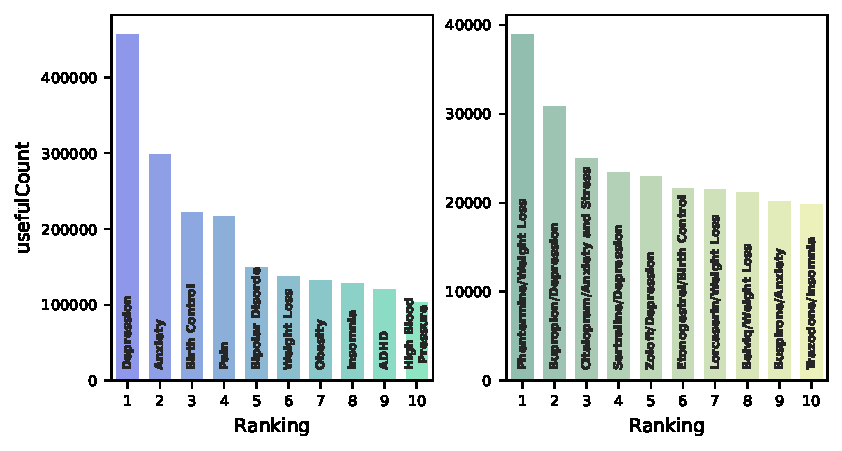
\includegraphics{plots/top_conditions.pdf}
\caption{Top 10 medical conditions by how useful the people found the reviews for their drugs \textit{(left)} and top 10 drugs along with medical conditions they are used for according to the same criteria \textit{(right)}.}
\label{fig:bars}
\centering
\end{figure}

%not sure how else to call this, maybe just "Word Occurrence and Ratings"
\subsection{Predicting ratings from word counts}

The simplest way of processing text is to count word occurrences and collect them in a vector, a "bag of words". In the following, we explore the importance of certain word counts for predicting the rating of a review. Although ratings are discrete, their semantics makes regression a more natural choice than classification. Predicting a rating of 8 when the true rating would be 2 is worse than predicting 3.\\
Figure \ref{fig:score_corr} shows the performance of linear regression models trained with word vectors containing one through fifty of the most common words in reviews of \textit{depression} medication. Performance is measured with the coefficient of determination R$^2$ \citep{wright1921correlation}, which has the advantage of accounting for the unconditional distribution of ratings. The best constant classifier has an R$^2$ value of 0. As expected, performance goes up with more information - we observed the same with more flexible models like decision trees, who reach an R$^2$ test score of approximately 0.7 with 50 input words.\\
The slope of the graph gives an indication of the importance of a word for the prediction, in particular, it shows the importance given preceding words. A steep slope here means that a word is important overall, but a shallow slope does not necessarily mean that it is not important. In this particular case, different permutations showed similar slopes at the same words.\\
In the background of Figure \ref{fig:score_corr}, the bar plot shows a measure of the absolute correlation between word occurrences and rating. Since review lengths are different for different ratings, we normalized word occurrences with text length. All important additional words for the regression have high correlations with ratings, but a high correlation doesn't mean a word is an important addition, because of correlation between words.


%One hurdle in interpreting correlation or the parameters of a model is different text lengths. If inputs are not normalized with text length 

%test scores better (?) - maybe speculate explanation
%words that are important for regressor not particularly high in correlation

%\begin{equation}
%    R^2 = 1- \frac{\sum_{i \in I} (y_i-\hat{y_i})^2}{\sum_{i \in I} (y_i-\bar{y})^2}
%\end{equation}


\begin{figure}[htb]
    \centering
    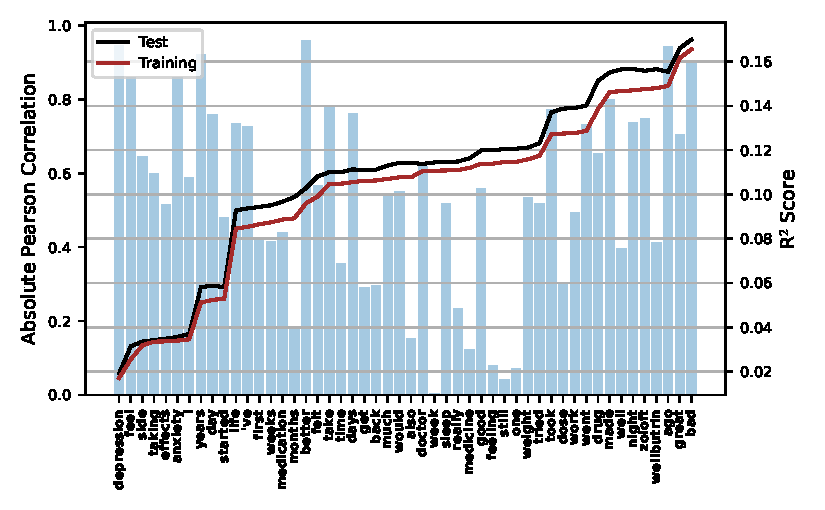
\includegraphics[width = \textwidth]{plots/score_corr_normalized.pdf}
    \caption{Lines show R$^2$ score of different linear models trained with word vectors containing words up to the ones labeling the x-axis; Bars show the absolute value of the Pearson correlation coefficient of word counts and ratings. Data is limited to the reviews for depression medications.\\
    The test score is a little better, which is likely a coincidence as the difference is very small and decision trees didn't show this behavior.}
    \label{fig:score_corr}
\end{figure}

\subsection{Sentiment analysis of reviews}

Sentiment analysis is an important task in all types of reviews as it helps in better understanding the emotion in the review and provides a possible direction for product improvements. This data is especially good for comparing the performance of different models on the task of sentiment analysis as it contains both the \emph{reviews} for medical drugs and the \emph{rating} from the user who wrote the review. We have separated the ratings in three different sentiment classes where \textit{class 0 = negative} is for $rating<5$, \textit{class 1 = neutral} for $rating=5$ and \textit{class 2 = positive} for $rating>5$. For the purpose of this task, we first evaluated all reviews using TextBlob Sentiment Analysis tool (?), using both filtered (removing stopwords and punctuation) and unfiltered reviews, and found the correlation between sentiment and grade is lower when using filtered data. The possible explanation for this is that word \textit{"not"} is among the stopwords, and when it is eliminated the sentiment might be predicted wrongly.\\
We have also compared the performance of three standard models: Random Forest \citep{randomForest}, Multinomial Naive Bayes \citep{mnb} and XGBoost \citep{xgboost}. All models were trained on test data and evaluated using test data where target classes were calculated as described previously. Since a classifier requires numeric input, the reviews were first converted to vectors using TF–IDF (term frequency-inverse document frequency) which is a term weighting scheme commonly used to represent textual documents as vectors \citep{tfidf}.\\
\begin{figure}[h!]
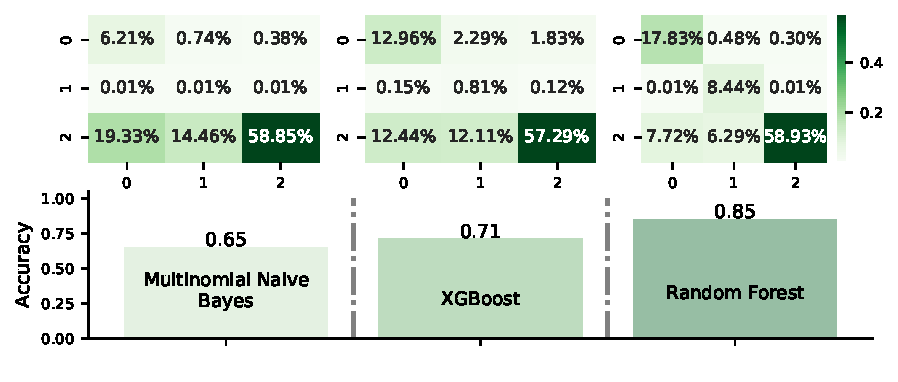
\includegraphics[width = \textwidth]{plots/sentiment_analysis.pdf}
\caption{Accuracy plot and Confusion Matrices for MNB, XGBoost and RF models where $0=negative, 1=neutral$ and $2=positive$ sentiment.} 
\label{fig:acc}
\centering
\end{figure}\\
The accuracy plot along with confusion matrices for all models can be seen in Figure \ref{fig:acc}. We can see that Random Forest outperforms all other models (with $85\%$ accuracy), even without any parameter tuning. We can tune the parameters of our classifier and improve the models' accuracy. Another important thing we can conclude is that all models seem to be better at predicting \textit{positive (class 2)} sentiment than \textit{negative (class 0)} and \textit{neutral (class 0)} sentiment. This is a consequence of the unbalanced number of samples of different classes - the largest number of samples in the training set comes from \textit{positive (class 2)} sentiment. In the future, we could try to balance the dataset using data augmentation: for example, changing some words with their synonyms because that would retain the sentiment of a review. This data augmentation could result in improving the accuracy.


\section{Conclusion}

We have shown a way of assessing the importance of word occurrences in a review for predicting the associated rating. Furthermore, we have also seen that the accuracy of commonly used sentiment analysis models is on an acceptable level for this task but could further be improved by balancing the dataset because there are more positive reviews than negative ones.
Identifying the sentiment of a review, and knowing which words might be important for
the rating can help us make an attempt at predicting the rating that the user would give to the given product and also help the pharmaceutical companies in better understanding the reaction of their
customers.
\printbibliography

\end{document}